\documentclass{standalone}
\usepackage{pgfplots}
\pgfplotsset{compat=1.18}

\begin{document}

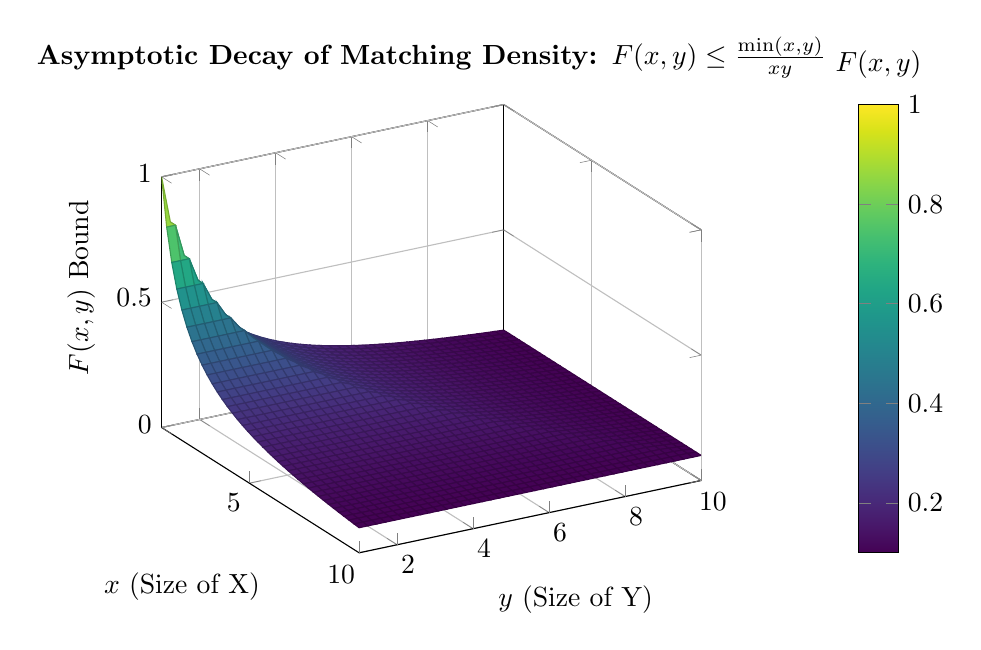
\begin{tikzpicture}
	\begin{axis}[
			title={\textbf{Asymptotic Decay of Matching Density: $F(x,y) \le \frac{\min(x,y)}{xy}$}},
			xlabel={$x$ (Size of X)},
			ylabel={$y$ (Size of Y)},
			zlabel={$F(x,y)$ Bound},
			xmin=1, xmax=10,
			ymin=1, ymax=10,
			zmin=0, zmax=1,
			grid=both,
			view={60}{30}, % Adjusts the 3D camera angle
			colormap/viridis, % Smooth color gradient from purple (low) to yellow (high)
			colorbar,
			colorbar style={title={$F(x,y)$}}
		]

		% Plot the upper bound function using the min(x,y)/(x*y) logic
		\addplot3[
			surf,
			domain=1:10,
			domain y=1:10,
			samples=40 % Increase for smoother surface, decrease if rendering is slow
		] { min(x,y) / (x*y) };

	\end{axis}
\end{tikzpicture}

\end{document}
